\section[Gruß von der anderen Seite (ein ehemaliger Physikstudent erzählt)]{Gruß von der anderen Seite\\(ein ehemaliger Physikstudent erzählt)}
\textbf{Ja, es gibt ein Leben nach dem Physikstudium, auch wenn viele von euch sich das aktuell sicher noch nicht vorstellen können.
Hier könnt ihr einen kurzen Einblick in das Leben von Johannes werfen.
Johannes war vor ein paar Jahren noch Physikstudent (Lehrämtler, heute 2FB) hier in Münster und hat sich mittlerweile über sein Referendariat zum Lehrer-Beruf durchgeschlagen.
Johannes (kurz JohPie) war zu seiner Zeit auch aktives Fachschafts-Mitglied und hat auch seine Höhen und Tiefen im Studium erlebt, aber lest selbst\dots}

\begin{multicols*}{2}
% XXX Das Bild ist schlimm!
\begin{wrapfigure}[10]{r}{0cm}
	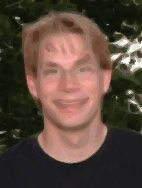
\includegraphics[width=3.1cm]{res/johannes_pieper.pdf}
\end{wrapfigure}
Vorweg: Herzlichen Glückwunsch zu eurer Entscheidung, ein Physikstudium in der lebenswerten Stadt Münster aufzunehmen.
Die gleiche Entscheidung habe ich auch getroffen und nun möchte ich etwas über meinen Weg an der Universität und dem anschließenden Referendariat erzählen.

Nach knapp acht Jahren, vielen Höhen und Tiefen habe ich endlich meine Ausbildung abgeschlossen.
Aber beginnen wir am Anfang.
Während des Zivildienstes habe ich die Entscheidung getroffen, Physik und Informatik auf Lehramt zu studieren.
Die Wahl einer Universität gestaltete sich schwieriger.
Einige Freunde von mir haben sich für Oldenburg entschieden, wo meine Fächerkombination aber nicht angeboten wurde.

Nach langem hin und her ist die Wahl auf Münster gefallen.
Dieses bot mir die Möglichkeit, in der Anfangszeit bei meinen Eltern wohnen zu bleiben, um von dort aus eine eigene Wohnung zu suchen.
In den ersten Wochen des Studiums zeigte sich aber schnell, dass das sehr schnell geschehen musste.
Die Fahrten zur Uni nahmen sehr viel Zeit in Anspruch und die Kontakte zu den anderen Studierenden waren erschwert.

\subsection{Studienbeginn}
Begonnen hat das Studium mit der Einschreibung im Münsteraner Schloss.
Alles war neu und man konnte nicht richtig überblicken, was auf einen zukommt.
Wahrscheinlich geht es euch sehr ähnlich.
Im Internet habe ich damals einen Hinweis auf die Ersti-Woche der Fachschaft Physik gefunden; dort gab es dann die ersten wichtigen Informationen zum Studium und, was viel wichtiger war, dort wurden die ersten Kontakte geknüpft.

Mit einem vollgepackten Stundenplan, in dem neben Physik, Informatik und Mathematik auch die Erziehungswissenschaften untergebracht werden mussten, ging es in die ersten Wochen des Studiums.
Während der erste Übungszettel noch einfach zu lösen war, wurde beim zweiten schon klar, dass ich allein auf mich gestellt dieses nicht lange durchhalten würde.
Die Lage entspannte sich etwas, nachdem ich eine WG gefunden hatte.
Am Ende des Semesters waren die Klausuren dicht gedrängt, aber mit dem nötigen Einsatz schaffbar.

Mit dem zweiten Semester wurde auch das Wetter in Münster wärmer und nun konnte ich nachvollziehen, warum alle vom Sommersemester schwärmten.
Es hat einfach ein besonderes Flair, wenn man sich nach der Vorlesung auf den Rasenflächen in der Sonne trifft oder abends am Aasee sitzt.

\subsection{Das dritte Semester ist das schwerste}
Zum Beginn des dritten Semesters änderte sich dann so einiges.
Als Erstes kam die Ersti-Woche, an der ich dieses Mal als Tutor teilgenommen habe.
Dabei bin ich stärker mit den Fachschaftlern in Kontakt gekommen, sodass ich anschließend die erste Fachschaftssitzung des neuen Semesters besucht habe.

Das dritte Semester hat aber auch den Ruf, das schwerste Semester zu sein.
Das gilt sowohl für Physik als auch für Informatik.
Neben dem Praktikum, bei dem man endlich selbst Versuche durchführen durfte, wurde der Stoff in der Physikvorlesung immer abstrakter und schwieriger.
Mein persönliches Resultat war das Nichtbestehen der Klausur am Ende des Semesters in Physik.
Dass ich damit zu etwa 60~Prozent meines Jahrgangs gehörte, war für mich kein großer Trost.

Die anschließende vorlesungsfreie Zeit war bei mir mit dem Lernen für die Klausur überschattet.
Unterbrochen wurde diese Zeit durch das Praktikum in der Schule, bei dem ich mich so wohl gefühlt habe, dass es mir weiteren Antrieb gegeben hat.
Außerdem habe ich die Chance ergriffen und in Informatik die Zwischenprüfung schon nach dem dritten Semester erfolgreich absolviert.

Aber dann kam die Wiederholungsklausur: Ein Blackout.
Ich saß in der Klausur und wusste nichts mehr, der Kopf war leer.
Am Ende habe ich ein leeres Blatt abgegeben und musste mich damit abfinden, dass ich im fünften Semester auch die Vorlesungen für das dritte Semester wieder besuchen müsste.
\begin{tikzpicture}[remember picture, overlay]
	\node[inner sep=0] at (current page.center)
	{\includegraphics[width=9cm]{private/res/kleeblatt.pdf}};
\end{tikzpicture}

\parshape=17
0cm \columnwidth
0cm \columnwidth
0cm \columnwidth
0cm \columnwidth
0cm \columnwidth
0cm \columnwidth
0cm 5.3cm
0cm 5cm
0cm 4.5cm
0cm 4.5cm
0cm 4.5cm
0cm 4.7cm
0cm 6.3cm
0cm 6.2cm
0cm 6.2cm
0cm 6.4cm
0cm \columnwidth
Dafür habe ich dann andere Dinge gemacht.
So war ich in meinem vierten Semester auch gleich Übungsgruppenleiter für die Informatik~4-Vorlesung und habe damit mein erstes Geld in der Uni verdient.
Entsprechend war ich auch am Ende des Semesters bei meiner ersten Klausurkorrektur dabei.
Mit dem Ende des Semester begann aber auch die Vorbereitung der neuen Ersti-Woche und ich hatte mich in der Fachschaft dazu bereit erklärt, die Koordination davon in die Hand zu nehmen.
Dieses setzte ich auch in den folgenden Jahren fort, genauso wie die Verantwortung für die Ersti-$\Phi$bel, von der du gerade einen Nachfolger in den Händen hältst.

\subsection{Hauptstudium}
\parshape=2
0cm 7.5cm
0cm \columnwidth
Mit dem Hauptstudium änderte sich so einiges im Studienverlauf.
Während im Grundstudium festgelegt war, was man zu besuchen hatte, konnte man nun zwischen vielen verschiedenen Angeboten wählen.
Dabei kam man stärker mit verschiedenen Professoren in Kontakt.

Während des Hauptstudiums gab es aber auch einige Vorlesungen, die wir besuchen mussten.
Bei diesen haben wir uns als Lehrämtler immer mehr gefragt, warum wir diese überhaupt besuchen sollten.
Einige der Themen würden wir nie in der Schule unterrichten.

Das Ende des Hauptstudiums wurde durch die Examensarbeit eingeläutet.
Die meisten Lehrämtler schreiben diese in der Didaktik der Physik.
Ich wollte aber noch einmal etwas von der aktuellen Forschung mitbekommen und bin in einer Arbeitsgruppe der Experimentellen Physik untergekommen.

\subsection{Examensprüfung}
Das Ende meines Studiums war vom Chaos des staatlichen Prüfungsamts überschattet.
Denn nachdem ich meine Examensklausuren geschrieben hatte, fehlte bei mir ein Termin der drei mündlichen Examensprüfungen.
Die dritte Prüfung fand dann erst nach dem Prüfungszeitraum statt, nachdem alle anderen ihre Prüfungen bereits beendet hatten.

\subsection{Referendariat}
\parshape=10
0cm \columnwidth
0cm \columnwidth
0cm \columnwidth
0cm \columnwidth
0cm \columnwidth
0cm \columnwidth
2.5cm \dimexpr\columnwidth - 2.5cm
3.3cm \dimexpr\columnwidth - 3.3cm
3.5cm \dimexpr\columnwidth - 3.5cm
0cm \columnwidth
Nach dem Studium ging es direkt über ins Referendariat.
Innerhalb des Referendariats habe ich dann festgestellt, dass die Dinge, deren Relevanz ich im Studium stark angezweifelt hatte, mir nun zusätzliche Sicherheit gaben.
Insgesamt habe ich aber auch im Referendariat Höhen und leider viel tiefere Tiefen als im Studium erlebt.
Aber nun bin ich fertiger Lehrer und bin zufrieden mit dem Ergebnis.

\subsection[Fazit]{\hspace{4.5cm}Fazit}
\parshape=9
4.5cm \dimexpr\columnwidth - 4.5cm
4.4cm \dimexpr\columnwidth - 4.4cm
4.2cm \dimexpr\columnwidth - 4.2cm
2cm \dimexpr\columnwidth - 2cm
4.2cm \dimexpr\columnwidth - 4.2cm
4.5cm \dimexpr\columnwidth - 4.5cm
4cm \dimexpr\columnwidth - 4cm
1.5cm \dimexpr\columnwidth - 1.5cm
0cm \columnwidth
Was bleibt am Ende festzuhalten?
Ein Physikstudium lohnt sich.
Es liefert einen breiten Einblick in eine spannende Wissenschaft.
Sehr wichtig ist es dabei, Kontakte zu knüpfen und zu halten.
Dieses gilt sowohl zu den Kommilitonen, als auch zu Professoren und Mitarbeitern.
Eine Sache würde ich aber ändern:
Wenn ich die Zeit zurückdrehen könnte, so würde ich mich für Physik auf Diplom (heute: Bachelor of Science \& Master of Science) statt Lehramt (heute: 2FB \& Master of Education) einschreiben.
Dank des Seiteneinstiegs kann man damit nach dem Studium immer noch sein Referendariat machen und Lehrer werden.
Sollte man aber nach der Uni feststellen, dass man doch nicht Lehrer werden will, so hat man immer noch einen eigenständigen Abschluss und nicht nur ein erstes Staatsexamen, was leider nichts zählt.

\begin{center}
	\Large\Fontlukas{Euch allen noch viel Erfolg bei eurem Physikstudium.}
\end{center}

\fibelsig{Johannes}
\end{multicols*}
